\documentclass[11pt,a4paper]{article}

\usepackage[utf8]{inputenc}
\usepackage[T1]{fontenc}
\usepackage[brazil]{babel}
\usepackage{amsmath,amssymb}
\usepackage{booktabs}
\usepackage{graphicx}
\usepackage{float}
\usepackage{geometry}
\usepackage{hyperref}
\usepackage{caption}
\usepackage{setspace}

\geometry{top=2.5cm, bottom=2.5cm, left=2.5cm, right=2.5cm}
\onehalfspacing

\title{\textbf{Análise de Regressão Linear Aplicada à Arrecadação de Doações da \textit{Loyal Order of Water Buffaloes}}}

\author{
  \textbf{[Nome Completo do(a) Integrante 1]} -- Matrícula: [XXXXXXXXX] \\
  \textbf{[Nome Completo do(a) Integrante 2]} -- Matrícula: [XXXXXXXXX] \\
  \small Departamento de Estatística -- Universidade Federal de Juiz de Fora (UFJF) \\
  \small EST074 -- Análise de Regressão (Classwork 06)
}

\date{13 de novembro de 2026}

\begin{document}

\maketitle

\begin{abstract}
Este trabalho tem como objetivo ajustar um modelo de regressão linear capaz de explicar o valor arrecadado em doações por reunião (\textit{Value}, em dólares) na organização \textit{Loyal Order of Water Buffaloes}, a partir do tipo de reunião (\textit{Meeting}), do número de membros presentes (\textit{Members}), do número de visitantes (\textit{Visitors}) e do total de participantes (\textit{Total}). A análise exploratória dos dados revelou forte assimetria positiva na variável resposta ($g_1 = 1{,}92$; $p < 0{,}001$), presença de valores atípicos e dependência linear exata entre o total de participantes e a soma de membros e visitantes, justificando a exclusão da variável \textit{Total} na modelagem. No ajuste do modelo linear completo, o tipo de reunião não apresentou significância estatística ao nível de 5\% ($p = 0{,}3358$), levando à adoção de um modelo reduzido apenas com membros e visitantes. O diagnóstico dos resíduos desse modelo inicial evidenciou violação da normalidade ($W = 0{,}863$; $p < 0{,}001$), dispersão crescente e observações influentes. Para contornar esses desvios, aplicou-se a transformação logarítmica na variável resposta ($\ln(\text{Value})$), reduzindo substancialmente a assimetria dos resíduos e melhorando a adequação do ajuste. No modelo final, mantendo as demais variáveis constantes, cada membro adicional associa-se a um aumento médio aproximado de $4{,}15\%$ no valor arrecadado ($p = 0{,}0015$), enquanto cada visitante adicional associa-se a um acréscimo médio de $2{,}53\%$ ($p < 0{,}001$).

\vspace{0.2cm}
\noindent\textbf{Palavras-chave:} Análise de regressão; Transformação logarítmica; Diagnóstico de resíduos; Assimetria; Arrecadação de doações.
\end{abstract}

\section{Introdução}

A \textit{Loyal Order of Water Buffaloes} é uma organização que realiza encontros periódicos nos quais são arrecadadas doações destinadas a ações de caridade. Compreender quais características das reuniões influenciam o montante arrecadado é relevante tanto para o planejamento de eventos futuros quanto para estimar o impacto da mobilização de membros e convidados sobre o volume de contribuições.

O conjunto de dados analisado é composto por 75 observações referentes a reuniões da organização e cinco variáveis: o valor arrecadado em dólares (\textit{Value}), que corresponde à variável resposta contínua; o tipo de reunião (\textit{Meeting}), variável qualitativa nominal com duas categorias (\textit{Ordinary} e \textit{Special}); o número de membros presentes (\textit{Members}); o número de visitantes presentes (\textit{Visitors}); e o número total de pessoas presentes (\textit{Total}). Na inspeção inicial da base, identificou-se que \textit{Value} apresenta seis valores ausentes e \textit{Visitors} apresenta um valor ausente, resultando em 69 observações completas para a etapa de regressão. Além disso, verificou-se que, em todos os registros válidos, o total de participantes corresponde exatamente à soma de membros e visitantes ($\text{Total} = \text{Members} + \text{Visitors}$).

Diante desse contexto, o objetivo deste trabalho é investigar o comportamento exploratório das variáveis disponíveis e ajustar um modelo de regressão linear adequado para explicar o valor arrecadado por reunião, avaliando a seleção de variáveis preditoras, os pressupostos do modelo por meio da análise de resíduos e a necessidade de transformação da variável resposta.

\section{Análise exploratória dos dados}

Inicialmente, analisou-se a distribuição da variável qualitativa \textit{Meeting}. Conforme apresentado na Tabela~\ref{tab:qualitativa} e ilustrado na Figura~\ref{fig:barras_meeting}, há predominância expressiva de reuniões ordinárias, que representam quase quatro quintos da amostra.

\begin{table}[H]
\centering
\caption{Distribuição de frequências da variável qualitativa \textit{Meeting}.}
\label{tab:qualitativa}
\begin{tabular}{lcc}
\toprule
\textbf{Categoria} & \textbf{Frequência absoluta ($n$)} & \textbf{Proporção (\%)} \\
\midrule
\textit{Ordinary} & 59 & 78,67\% \\
\textit{Special}  & 16 & 21,33\% \\
\midrule
\textbf{Total}    & \textbf{75} & \textbf{100,00\%} \\
\bottomrule
\end{tabular}
\end{table}

\begin{figure}[H]
\centering
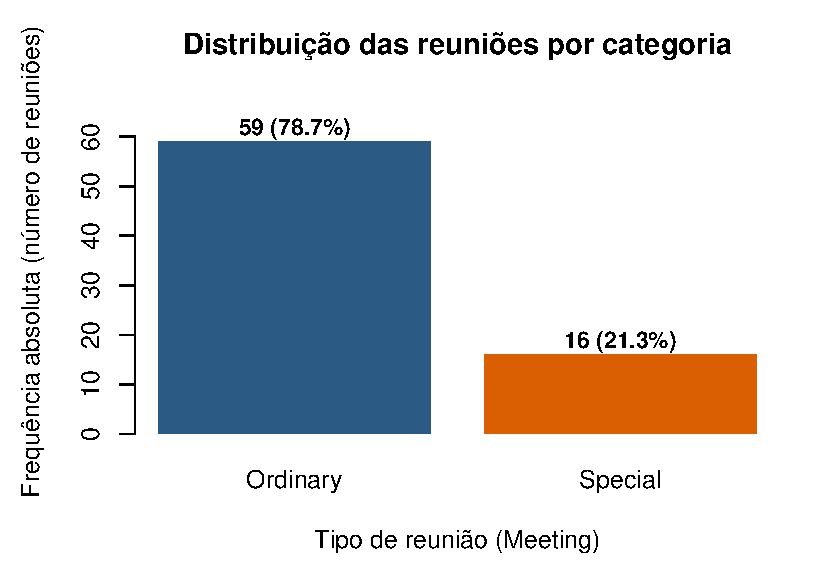
\includegraphics[width=0.62\textwidth]{figuras/fig1_barras_meeting.pdf}
\caption{Gráfico de barras com a contagem e o percentual de reuniões por categoria.}
\label{fig:barras_meeting}
\end{figure}

As medidas descritivas das quatro variáveis quantitativas encontram-se reunidas na Tabela~\ref{tab:descritivas}. O valor arrecadado (\textit{Value}) apresentou média de US\$~143,81 e mediana de US\$~123,00, com desvio padrão de US\$~75,09 e coeficiente de variação de 52,21\%, sinalizando dispersão elevada e concentração de observações em valores moderados acompanhada por uma cauda superior longa (máximo de US\$~392,00). O número de membros (\textit{Members}) mostrou comportamento mais homogêneo (média de 22,12, mediana de 22,00 e coeficiente de variação de 17,24\%). Por sua vez, o número de visitantes (\textit{Visitors}) exibiu variabilidade acentuada (coeficiente de variação de 177,35\%), com mediana de apenas 2 visitantes e máximo atípico de 65 visitantes. Esse pico também se reflete na variável \textit{Total}, cujo máximo atingiu 89 participantes frente a uma mediana de 25.

\begin{table}[H]
\centering
\caption{Medidas descritivas das variáveis quantitativas analisadas.}
\label{tab:descritivas}
\resizebox{\textwidth}{!}{%
\begin{tabular}{lccccccccc}
\toprule
\textbf{Variável} & \textbf{$n$} & \textbf{Média} & \textbf{Mediana} & \textbf{$Q_1$} & \textbf{$Q_3$} & \textbf{Mínimo} & \textbf{Máximo} & \textbf{Desvio Padrão} & \textbf{CV (\%)} \\
\midrule
\textit{Value} (US\$) & 69 & 143,81 & 123,00 & 97,75 & 152,00 & 57,00 & 392,00 & 75,09 & 52,21 \\
\textit{Members}      & 75 & 22,12  & 22,00  & 19,50 & 25,00  & 10,00 & 32,00  & 3,81  & 17,24 \\
\textit{Visitors}     & 74 & 5,61   & 2,00   & 1,00  & 5,00   & 0,00  & 65,00  & 9,95  & 177,35 \\
\textit{Total}        & 75 & 27,65  & 25,00  & 22,00 & 28,50  & 10,00 & 89,00  & 11,56 & 41,81 \\
\bottomrule
\end{tabular}%
}
\end{table}

Os histogramas e box-plots da Figura~\ref{fig:hist_box} confirmam visualmente esses padrões: enquanto \textit{Members} apresenta distribuição aproximadamente simétrica em torno de 22 membros (com apenas um ponto atípico inferior igual a 10), \textit{Value}, \textit{Visitors} e \textit{Total} exibem forte assimetria à direita e múltiplos valores atípicos superiores.

\begin{figure}[H]
\centering
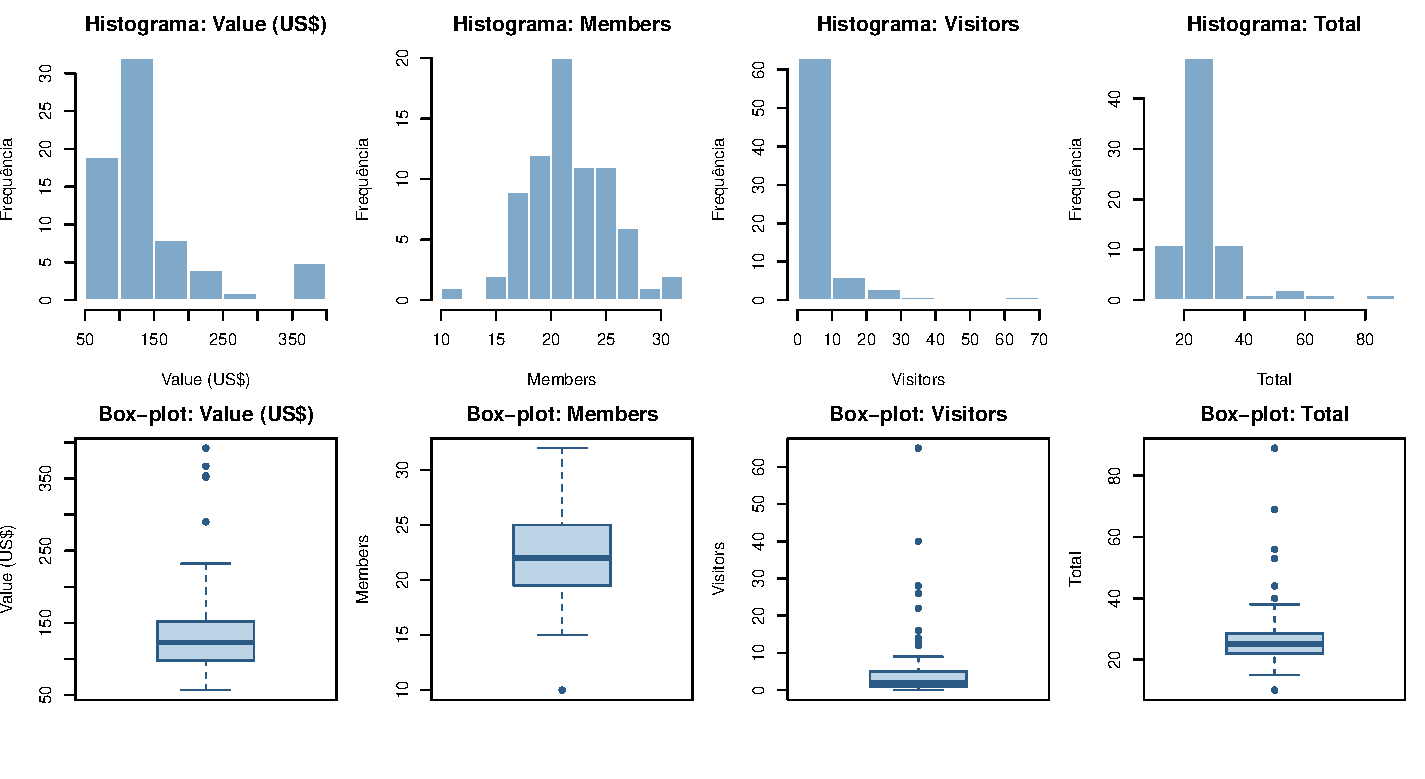
\includegraphics[width=0.98\textwidth]{figuras/fig2_hist_box_quant.pdf}
\caption{Histogramas e box-plots das variáveis quantitativas \textit{Value}, \textit{Members}, \textit{Visitors} e \textit{Total}.}
\label{fig:hist_box}
\end{figure}

Para investigar formalmente a assimetria e a aderência à distribuição normal da variável resposta, aplicou-se o teste $z$ assintótico de assimetria e o teste de Shapiro-Wilk, tanto nos dados originais quanto após a transformação logarítmica natural ($\ln(\text{Value})$), além da estratificação por tipo de reunião. Os resultados estão sumarizados na Tabela~\ref{tab:normalidade} e ilustrados na Figura~\ref{fig:value_log_meeting}.

\begin{table}[H]
\centering
\caption{Testes de assimetria e normalidade (Shapiro-Wilk) para \textit{Value} e $\ln(\text{Value})$, globalmente e por categoria de \textit{Meeting}.}
\label{tab:normalidade}
\begin{tabular}{llcc}
\toprule
\textbf{Variável / Escala} & \textbf{Escopo / Teste} & \textbf{Estatística} & \textbf{Valor-$p$} \\
\midrule
\textit{Value} (original) & Assimetria global ($g_1$)       & $g_1 = 1{,}922$ ($z = 6{,}517$) & $< 0{,}0001$ \\
\textit{Value} (original) & Shapiro-Wilk global             & $W = 0{,}752$                   & $< 0{,}0001$ \\
\textit{Value} (original) & Shapiro-Wilk -- \textit{Ordinary} & $W = 0{,}741$                 & $< 0{,}0001$ \\
\textit{Value} (original) & Shapiro-Wilk -- \textit{Special}  & $W = 0{,}747$                 & $0{,}0025$ \\
\midrule
$\ln(\text{Value})$       & Assimetria global ($g_1$)       & $g_1 = 0{,}889$ ($z = 3{,}013$) & $0{,}0026$ \\
$\ln(\text{Value})$       & Shapiro-Wilk global             & $W = 0{,}927$                   & $0{,}0006$ \\
$\ln(\text{Value})$       & Shapiro-Wilk -- \textit{Ordinary} & $W = 0{,}922$                 & $0{,}0012$ \\
$\ln(\text{Value})$       & Shapiro-Wilk -- \textit{Special}  & $W = 0{,}890$                 & $0{,}1167$ \\
\bottomrule
\end{tabular}
\end{table}

Na escala original, \textit{Value} apresenta assimetria positiva acentuada ($g_1 = 1{,}922$; $p < 0{,}0001$) e rejeição contundente da normalidade tanto no conjunto completo ($W = 0{,}752$) quanto em ambas as categorias de reunião. Ao aplicar o logaritmo natural, a assimetria cai para menos da metade ($g_1 = 0{,}889$), o gráfico Q-Q aproxima-se consideravelmente da reta teórica (Figura~\ref{fig:value_log_meeting}) e o grupo \textit{Special} passa a não rejeitar a hipótese de normalidade ao nível de 5\% ($W = 0{,}890$; $p = 0{,}1167$). Adicionalmente, realizou-se um teste $t$ de Welch comparando as médias de $\ln(\text{Value})$ entre reuniões ordinárias ($\bar{y}_{\text{Ord}} = 4{,}843$) e especiais ($\bar{y}_{\text{Esp}} = 4{,}999$), não sendo encontrada diferença estatisticamente significativa entre os grupos ($t = -1{,}330$; $\text{gl} = 18{,}48$; $p = 0{,}1997$; IC~95\% para a diferença: $[-0{,}402;\; 0{,}090]$).

\begin{figure}[H]
\centering
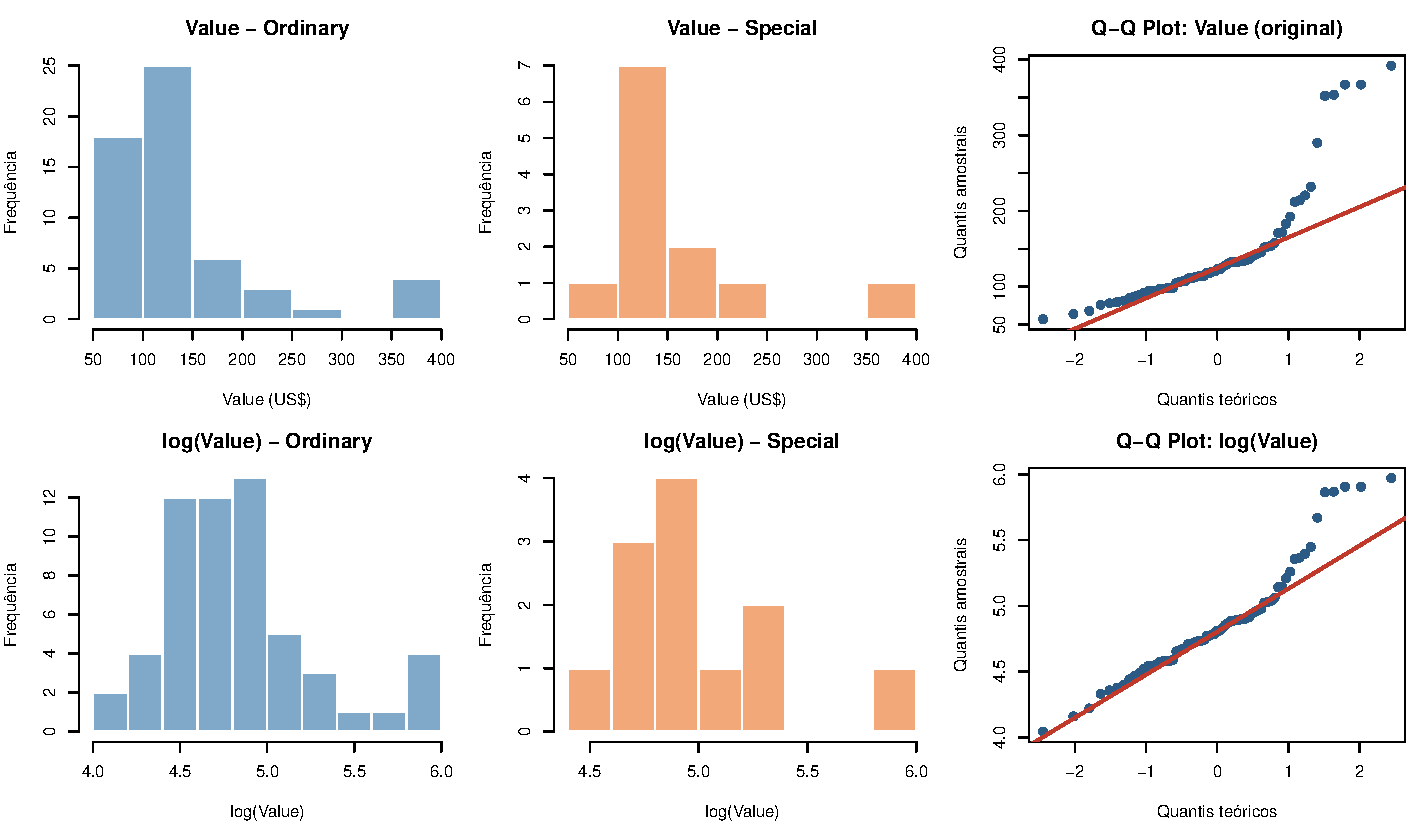
\includegraphics[width=0.98\textwidth]{figuras/fig3_value_log_meeting.pdf}
\caption{Comparação da distribuição de \textit{Value} (linha superior) e $\ln(\text{Value})$ (linha inferior) por tipo de reunião e respectivos Q-Q plots.}
\label{fig:value_log_meeting}
\end{figure}

A Figura~\ref{fig:matriz_disp} apresenta a matriz de dispersão envolvendo todas as variáveis do estudo, com histogramas na diagonal principal e coeficientes de correlação de Pearson no triângulo superior. Observa-se associação linear positiva moderada de \textit{Value} com \textit{Members} ($r = 0{,}49$), \textit{Visitors} ($r = 0{,}53$) e \textit{Total} ($r = 0{,}63$). Nota-se também correlação extremamente alta entre \textit{Visitors} e \textit{Total} ($r = 0{,}95$), consequência direta da identidade algébrica $\text{Total} = \text{Members} + \text{Visitors}$. Esse resultado reforça que a inclusão simultânea das três variáveis de contagem em um mesmo modelo geraria multicolinearidade perfeita, inviabilizando a estimação individual dos parâmetros. Além disso, a dispersão confirma a existência de observações atípicas com arrecadação elevada (acima de US\$~350) mesmo com poucos visitantes, bem como reuniões com número expressivo de visitantes (40 e 65 visitantes).

\begin{figure}[H]
\centering
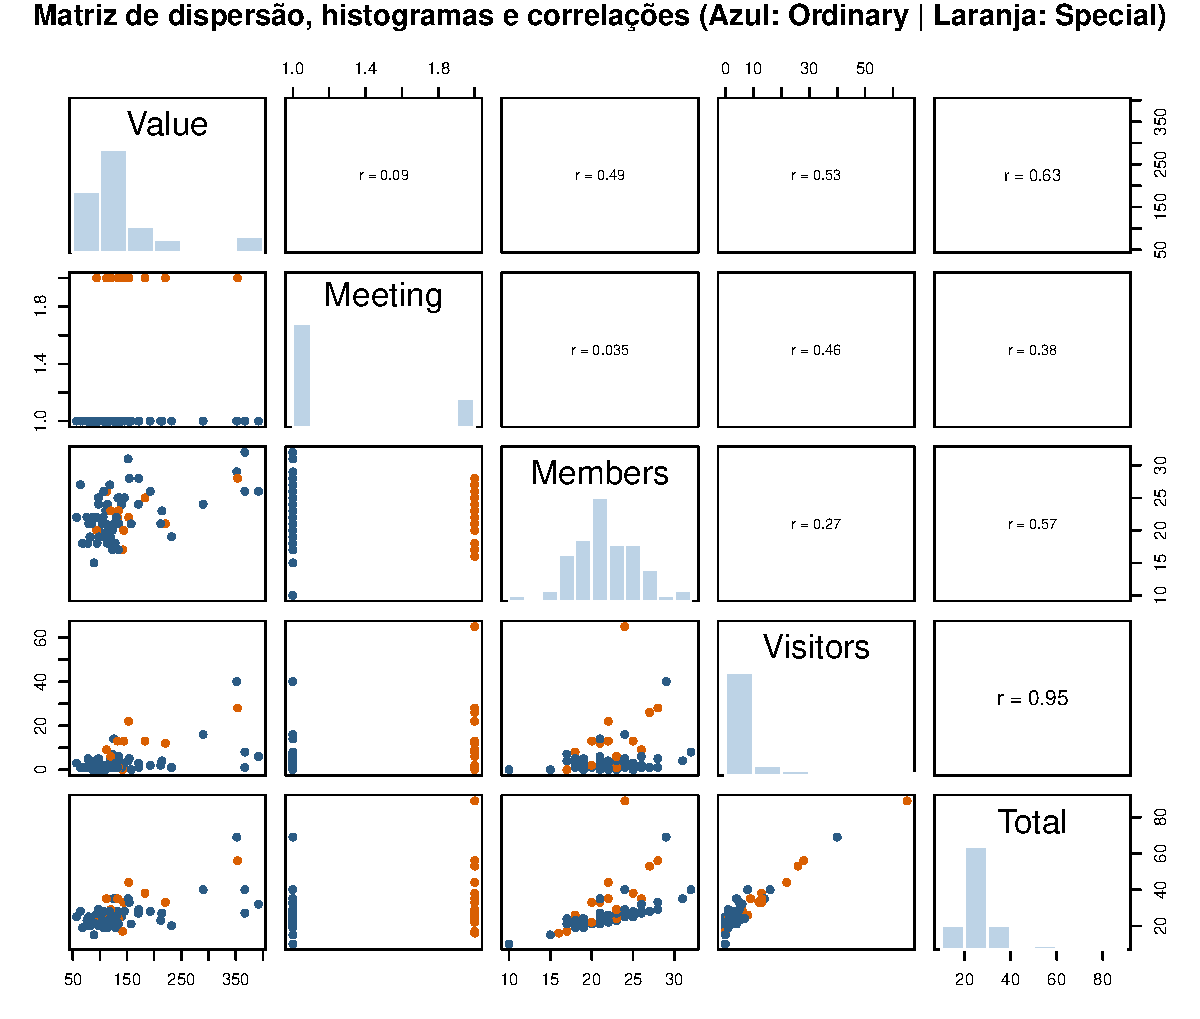
\includegraphics[width=0.88\textwidth]{figuras/fig4_matriz_dispersao.pdf}
\caption{Matriz de dispersão entre todas as variáveis (Azul: \textit{Ordinary}; Laranja: \textit{Special}), com histogramas na diagonal e correlações de Pearson no triângulo superior.}
\label{fig:matriz_disp}
\end{figure}

\section{Modelo de regressão}

\subsection{Seleção de variáveis, modelo completo e modelo reduzido}

Para explicar a variável resposta \textit{Value} (em dólares), consideraram-se como candidatas as variáveis preditoras \textit{Meeting} (tendo \textit{Ordinary} como categoria de referência e a variável indicadora \textit{MeetingSpecial} igual a 1 para reuniões especiais), \textit{Members} e \textit{Visitors}. A variável \textit{Total} foi excluída antes do ajuste por ser uma combinação linear exata de \textit{Members} e \textit{Visitors}. O ajuste foi realizado sobre as 69 observações com registros completos.

No modelo completo ajustado inicialmente:
\[
\widehat{\text{Value}} = -45{,}911 - 19{,}552\,\text{MeetingSpecial} + 7{,}603\,\text{Members} + 5{,}094\,\text{Visitors},
\]
obteve-se coeficiente de determinação $R^2 = 0{,}4122$ ($R^2_{\text{ajust}} = 0{,}3851$), erro padrão residual de $58{,}88$ e estatística global $F = 15{,}19$ ($\text{gl} = 3$ e $65$; $p = 1{,}35 \times 10^{-7}$). Conforme detalhado na Tabela~\ref{tab:modelos_originais}, os coeficientes de \textit{Members} ($p = 0{,}0007$) e \textit{Visitors} ($p < 0{,}0001$) mostraram-se altamente significativos ao nível de 5\%, ao passo que \textit{MeetingSpecial} não apresentou significância estatística ($p = 0{,}3358$).

\begin{table}[H]
\centering
\caption{Estimativas dos coeficientes dos modelos completo e reduzido na escala original (\textit{Value}).}
\label{tab:modelos_originais}
\begin{tabular}{lcccc}
\toprule
\textbf{Termo} & \textbf{Estimativa ($\hat{\beta}$)} & \textbf{Erro Padrão} & \textbf{Estatística $t$} & \textbf{Valor-$p$} \\
\midrule
\multicolumn{5}{l}{\textit{Modelo Completo} ($R^2 = 0{,}4122$; $R^2_{\text{ajust}} = 0{,}3851$; $F = 15{,}19$; $p = 1{,}35 \times 10^{-7}$)} \\
Intercepto              & $-45{,}911$ & $47{,}037$ & $-0{,}976$ & $0{,}3327$ \\
\textit{MeetingSpecial} & $-19{,}552$ & $20{,}164$ & $-0{,}970$ & $0{,}3358$ \\
\textit{Members}        & $7{,}603$   & $2{,}134$  & $3{,}562$  & $0{,}0007$ \\
\textit{Visitors}       & $5{,}094$   & $1{,}189$  & $4{,}285$  & $< 0{,}0001$ \\
\midrule
\multicolumn{5}{l}{\textit{Modelo Reduzido} ($R^2 = 0{,}4037$; $R^2_{\text{ajust}} = 0{,}3856$; $F = 22{,}34$; $p = 3{,}90 \times 10^{-8}$)} \\
Intercepto              & $-50{,}394$ & $46{,}787$ & $-1{,}077$ & $0{,}2854$ \\
\textit{Members}        & $7{,}739$   & $2{,}129$  & $3{,}635$  & $0{,}0005$ \\
\textit{Visitors}       & $4{,}667$   & $1{,}104$  & $4{,}228$  & $< 0{,}0001$ \\
\bottomrule
\end{tabular}
\end{table}

Em virtude da não significância do tipo de reunião — resultado coerente com o teste $t$ exploratório que tampouco indicou diferença média relevante entre os tipos de encontro —, propôs-se o modelo reduzido contendo apenas \textit{Members} e \textit{Visitors}. O teste $F$ parcial comparando o modelo reduzido ao completo confirmou que a exclusão de \textit{Meeting} não provoca perda significativa de poder explicativo ($F = 0{,}940$; $p = 0{,}3358$), chegando inclusive a elevar ligeiramente o $R^2_{\text{ajust}}$ de $0{,}3851$ para $0{,}3856$.

\subsection{Análise de resíduos e transformação da variável resposta}

A verificação dos pressupostos do modelo reduzido na escala original (Figura~\ref{fig:diag_original}) revelou desvios importantes. No gráfico de resíduos versus valores ajustados e no gráfico escala-localização, nota-se tendência de dispersão crescente para valores ajustados intermediários e resíduos positivos muito elevados (superiores a US\$~200). No gráfico Q-Q normal, os quantis superiores afastam-se fortemente da reta teórica, o que é corroborado pelo teste de Shapiro-Wilk sobre os resíduos ($W = 0{,}8633$; $p = 2{,}09 \times 10^{-6}$) e pela assimetria residual positiva ($g_1 = 1{,}636$). Além disso, o gráfico da distância de Cook destaca as observações 62 ($D = 0{,}282$), 60 ($D = 0{,}197$) e 70 ($D = 0{,}143$), correspondentes a reuniões ordinárias com arrecadações entre US\$~367,00 e US\$~392,00 muito acima do previsto pelo número de participantes.

\begin{figure}[H]
\centering
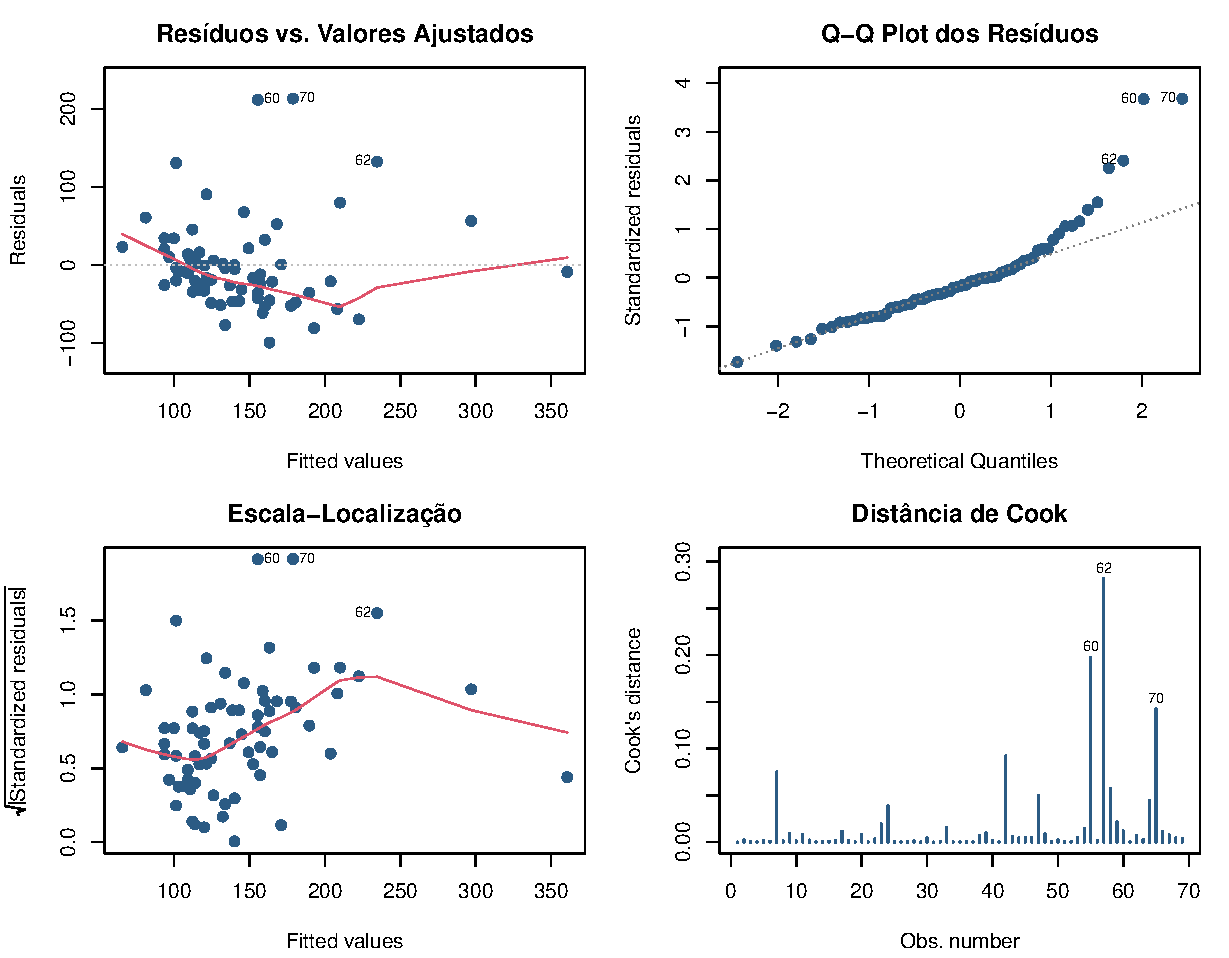
\includegraphics[width=0.92\textwidth]{figuras/fig5_diagnostico_original.pdf}
\caption{Gráficos de diagnóstico dos resíduos do modelo reduzido na escala original (\textit{Value}).}
\label{fig:diag_original}
\end{figure}

Em consonância com a forte assimetria positiva identificada ainda na análise exploratória, aplicou-se a transformação logarítmica natural à variável resposta, passando a modelar $\ln(\text{Value})$. Inicialmente ajustou-se o modelo completo transformado, no qual o termo \textit{MeetingSpecial} permaneceu não significativo ($\hat{\beta} = -0{,}0331$; $p = 0{,}7786$; teste $F$ parcial $= 0{,}0797$; $p = 0{,}7786$). Dessa forma, manteve-se a estrutura reduzida com \textit{Members} e \textit{Visitors}, cujos resultados constam na Tabela~\ref{tab:modelo_log}.

\begin{table}[H]
\centering
\caption{Estimativas dos coeficientes do modelo final transformado ($\ln(\text{Value})$).}
\label{tab:modelo_log}
\begin{tabular}{lcccc}
\toprule
\textbf{Termo} & \textbf{Estimativa ($\hat{\beta}$)} & \textbf{Erro Padrão} & \textbf{Estatística $t$} & \textbf{Valor-$p$} \\
\midrule
\multicolumn{5}{l}{\textit{Modelo Final Reduzido} ($R^2 = 0{,}3645$; $R^2_{\text{ajust}} = 0{,}3452$; $F = 18{,}93$; $p = 3{,}19 \times 10^{-7}$)} \\
Intercepto       & $3{,}8473$ & $0{,}2699$ & $14{,}252$ & $< 0{,}0001$ \\
\textit{Members} & $0{,}0407$ & $0{,}0123$ & $3{,}312$  & $0{,}0015$ \\
\textit{Visitors}& $0{,}0250$ & $0{,}0064$ & $3{,}923$  & $0{,}0002$ \\
\bottomrule
\end{tabular}
\end{table}

Os gráficos diagnósticos do modelo com resposta log-transformada (Figura~\ref{fig:diag_log}) demonstram melhora substancial na adequação do ajuste. A linha suavizada no gráfico de resíduos versus valores ajustados torna-se mais próxima de zero e a variância mostra-se mais estável ao longo dos valores ajustados. No Q-Q plot, os pontos alinham-se melhor à reta teórica: a assimetria dos resíduos cai de $1{,}636$ para $0{,}574$ e a estatística de Shapiro-Wilk sobe de $W = 0{,}8633$ para $W = 0{,}9590$ ($p = 0{,}0236$). Adicionalmente, a influência das observações extremas é atenuada, com a maior distância de Cook reduzida quase pela metade (observação 62 com $D = 0{,}149$, seguida pela observação 60 com $D = 0{,}126$ e observação 63 com $D = 0{,}116$).

\begin{figure}[H]
\centering
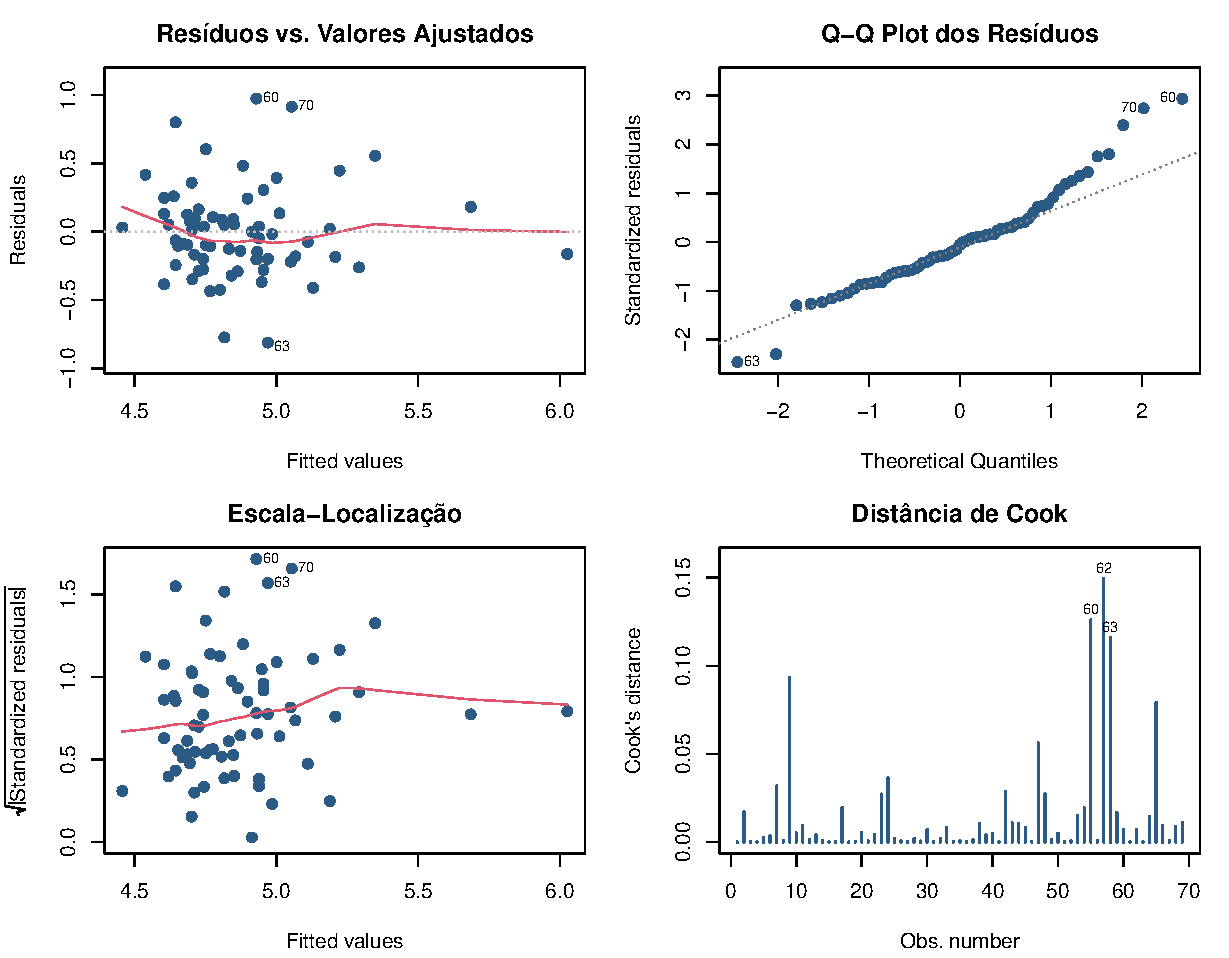
\includegraphics[width=0.92\textwidth]{figuras/fig6_diagnostico_log.pdf}
\caption{Gráficos de diagnóstico dos resíduos do modelo final com variável resposta transformada ($\ln(\text{Value})$).}
\label{fig:diag_log}
\end{figure}

\subsection{Interpretação dos coeficientes do modelo final}

A equação estimada do modelo final é dada por:
\[
\widehat{\ln(\text{Value})} = 3{,}8473 + 0{,}0407\,\text{Members} + 0{,}0250\,\text{Visitors},
\]
ou, de forma equivalente na escala monetária original (mediante exponenciação),
\[
\widehat{\text{Value}} = \exp(3{,}8473) \cdot \exp(0{,}0407\,\text{Members}) \cdot \exp(0{,}0250\,\text{Visitors}).
\]

A interpretação dos efeitos parciais, mantendo as demais variáveis constantes, ocorre de maneira multiplicativa (percentual):
\begin{itemize}
    \item \textbf{Intercepto ($\hat{\beta}_0 = 3{,}8473$; $p < 0{,}0001$):} corresponde ao logaritmo natural esperado do valor arrecadado quando o número de membros e de visitantes é igual a zero ($\exp(3{,}8473) \approx \text{US\$}~46{,}87$). Embora matematicamente necessário ao ajuste, não possui interpretação prática direta, pois nenhuma reunião registrada ocorreu sem participantes.
    \item \textbf{Efeito de \textit{Members} ($\hat{\beta}_1 = 0{,}0407$; $p = 0{,}0015$):} o sinal positivo indica que reuniões com maior número de membros tendem a arrecadar mais. Mantendo o número de visitantes constante, cada membro adicional aumenta $\ln(\text{Value})$ em $0{,}0407$ unidades, o que equivale a um acréscimo médio estimado de $\exp(0{,}04068) - 1 \approx 4{,}15\%$ no valor arrecadado por reunião. A título comparativo, no modelo sem transformação esse efeito correspondia a um aumento médio linear de US\$~7,74 por membro adicional.
    \item \textbf{Efeito de \textit{Visitors} ($\hat{\beta}_2 = 0{,}0250$; $p = 0{,}0002$):} o sinal positivo confirma que a presença de visitantes também contribui significativamente para elevar as doações. Mantendo o número de membros constante, cada visitante adicional aumenta $\ln(\text{Value})$ em $0{,}0250$ unidades, representando um incremento médio de $\exp(0{,}02498) - 1 \approx 2{,}53\%$ no valor arrecadado (frente a US\$~4,67 por visitante no modelo linear original). Nota-se que o impacto marginal de um membro adicional é superior ao de um visitante adicional.
\end{itemize}

O modelo final apresenta significância estatística global ($F = 18{,}93$; $p = 3{,}19 \times 10^{-7}$) e explica aproximadamente $36{,}45\%$ da variabilidade de $\ln(\text{Value})$ ($R^2_{\text{ajust}} = 34{,}52\%$), indicando que, embora a composição de participantes seja um determinante relevante da arrecadação, outros fatores não observados no banco de dados também influenciam o valor doado em cada encontro.

\section{Conclusão}

Neste trabalho, analisou-se o comportamento das doações arrecadadas pela \textit{Loyal Order of Water Buffaloes} e ajustou-se um modelo de regressão linear para explicar o valor obtido por reunião. A análise exploratória evidenciou a redundância estrutural da variável \textit{Total} ($\text{Members} + \text{Visitors}$) e a acentuada assimetria positiva da variável resposta \textit{Value} ($g_1 = 1{,}922$), além da ausência de diferença estatisticamente significativa entre reuniões ordinárias e especiais.

Na modelagem estatística, a exclusão de \textit{Meeting} foi justificada tanto pela ausência de significância individual quanto pelo teste $F$ parcial ($p = 0{,}3358$). O diagnóstico dos resíduos do modelo original apontou forte não normalidade e presença de observações influentes, motivando a adoção da transformação logarítmica $\ln(\text{Value})$, que reduziu a assimetria residual de $1{,}636$ para $0{,}574$ e atenuou a influência de pontos extremos. O modelo final evidenciou que tanto o número de membros quanto o número de visitantes exercem efeitos positivos e estatisticamente significativos sobre a arrecadação (aumentos médios de $4{,}15\%$ por membro e $2{,}53\%$ por visitante, mantendo a outra variável constante), fornecendo subsídio quantitativo para que a organização priorize o engajamento de seus membros e o convite a novos visitantes em suas reuniões beneficentes.

\begin{thebibliography}{9}

\bibitem{montgomery2021}
MONTGOMERY, D. C.; PECK, E. A.; VINING, G. G. \textit{Introduction to Linear Regression Analysis}. 6. ed. Hoboken: John Wiley \& Sons, 2021.

\bibitem{kutner2005}
KUTNER, M. H.; NACHTSHEIM, C. J.; NETER, J.; LI, W. \textit{Applied Linear Statistical Models}. 5. ed. Boston: McGraw-Hill/Irwin, 2005.

\bibitem{faraway2014}
FARAWAY, J. J. \textit{Linear Models with R}. 2. ed. Boca Raton: Chapman and Hall/CRC, 2014.

\end{thebibliography}

\end{document}
